\section{Akselerator Perangkat Keras untuk \acl{RL}}
\label{sec:accelerator-researches}

Sebelum penelitian tugas akhir ini, terdapat beberapa pengembangan akselerator perangkat keras untuk \ac{RL} yang diimplementasikan pada \ac{FPGA}. Berdasarkan \parencite{sutisna2023faraneq}, pengembangan akselerator perangkat keras untuk \ac{RL} menggunakan teknik \textit{Q-Learning} itu pertama kali dikembangkan oleh Da Silva et al pada \parencite{dasilva2019parallel}. Implementasi yang dikembangkan pada \parencite{dasilva2019parallel} berfokus untuk mengoptimalisasi perhitungan pada persamaan \ref{eq:q-learning} menggunakan teknik perhitungan paralel yang diilustrasikan pada gambar \ref{fig:ilustrasi-dasilvi}.

\begin{figure}[h]
	\centering
	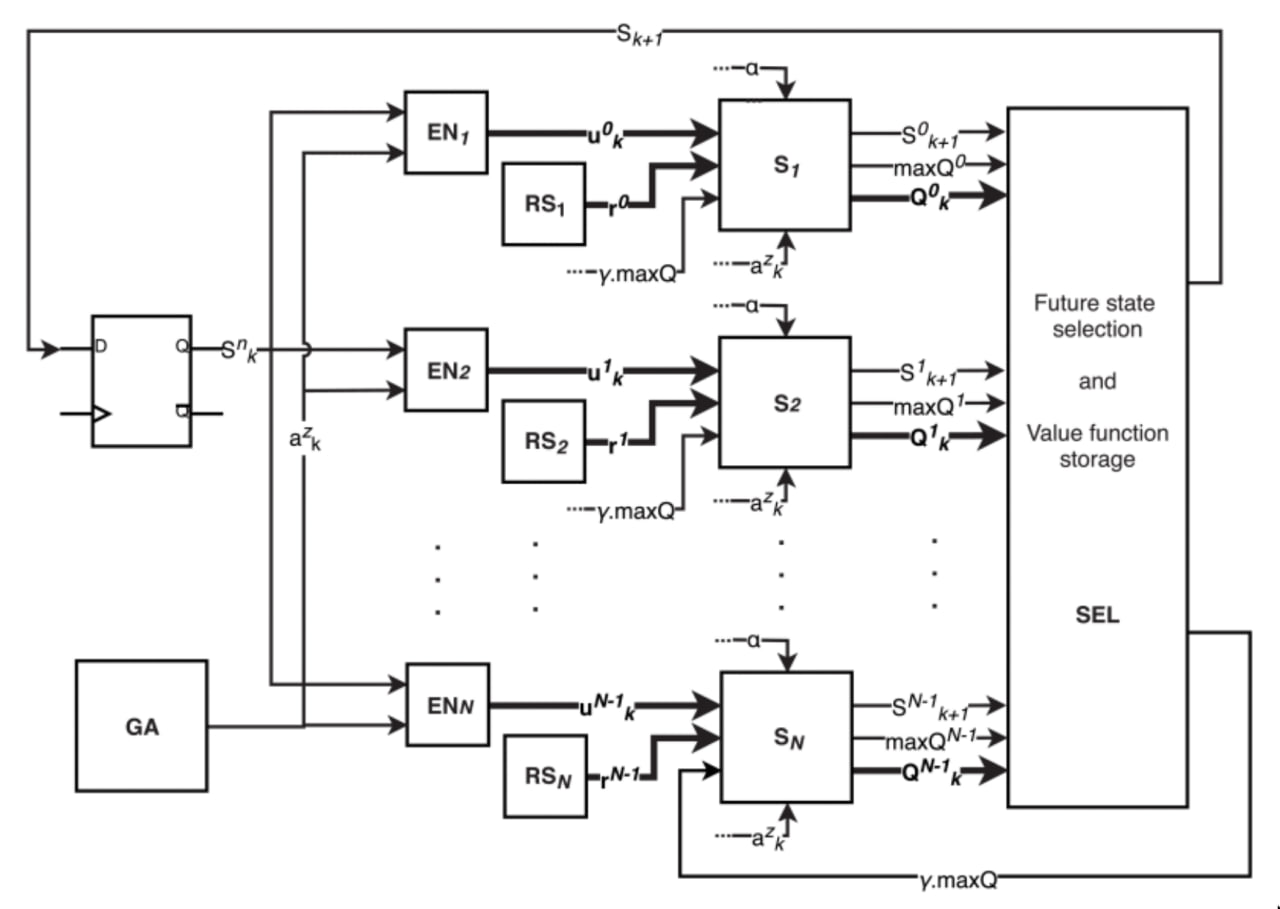
\includegraphics[width=0.8\textwidth]{chapter-2/dasilvi.jpg}
	\caption{Ilustrasi teknik perhitungan paralel \parencite{dasilva2019parallel}}
	\label{fig:ilustrasi-dasilvi}
\end{figure}

Teknik perhitungan paralel tersebut berhasil mendapat kecepatan \textit{throughput} sebesar 13.4  \ac{MSps} untuk \textit{Q-Table} yang memiliki 132 \textit{state} dan 4 aksi. Lalu, ada pula implementasi akselerator perangkat keras dari Spanò et al \parencite{spano2019efficient}. Arsitektur akselerator perangkat keras yang dikembangkan oleh \parencite{spano2019efficient} merupakan akselerator yang memanfaatkan penggunaan \textit{internal} \ac{RAM} \textit{block} untuk menyimpan \textit{Q-Table} dan melakukan perhitungan pada persamaan \ref{eq:q-learning} secara simultan. Gambar \ref{fig:ilustrasi-spano} menggambarkan arsitektur yang dirancang oleh \parencite{spano2019efficient}.

\begin{figure}[h]
	\centering
	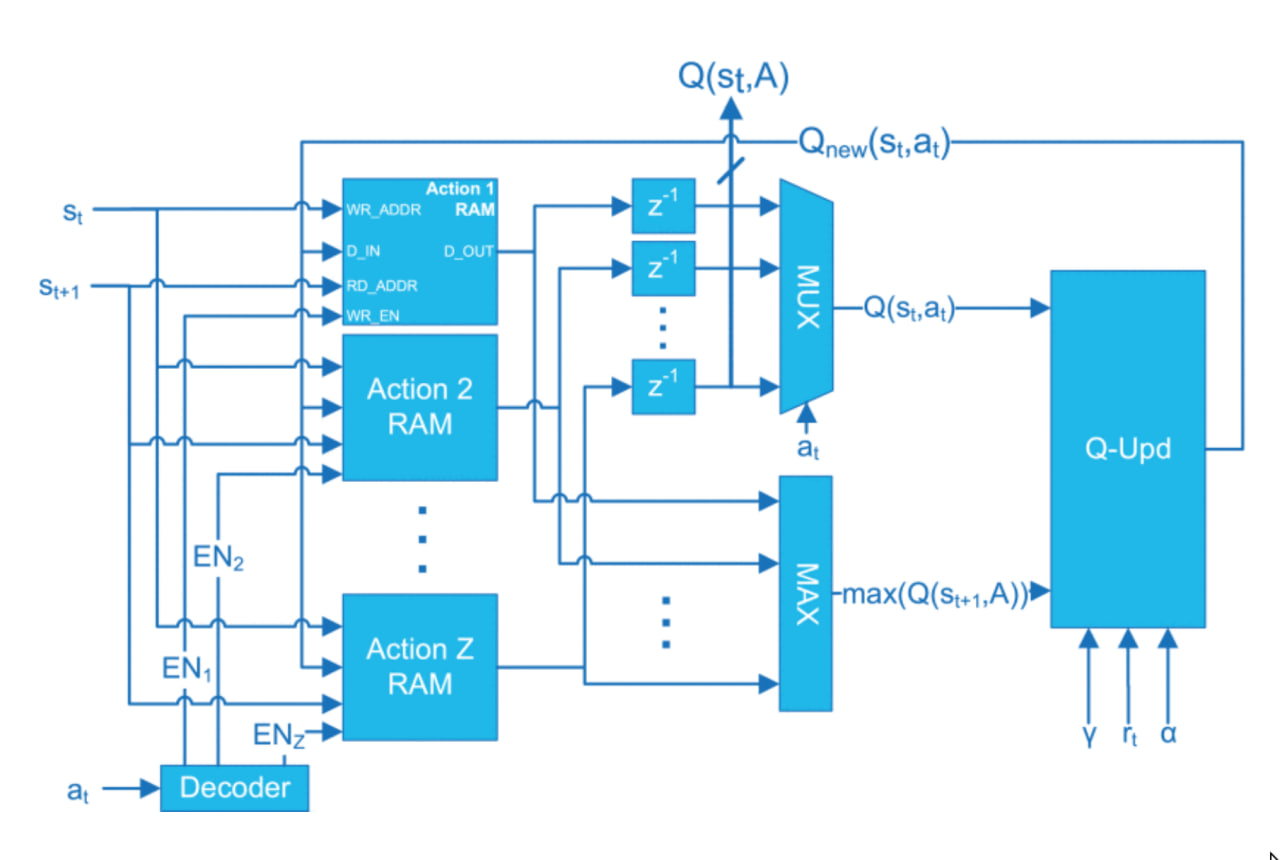
\includegraphics[width=0.8\textwidth]{chapter-2/spano.jpg}
	\caption{Ilustrasi arsitektur akselerator \parencite{spano2019efficient}}
	\label{fig:ilustrasi-spano}
\end{figure}

Akselerator perangkat keras dari \parencite{spano2019efficient} berhasil mendapatkan kecepatan \textit{throughput} sebesar 112 MSps untuk \textit{Q-Table} dengan 128 \textit{state} and 4 aksi. Arsitektur yang dikembangkan oleh \parencite{spano2019efficient}, merupakan akselerator \textit{Q-Learning} yang dapat digunakan secara \textit{Generic} karena implementasinya memberikan fleksibilitas kepada pengguna akselerator untuk membangun desain lingkungan agen \ac{RL}.

Pengembangan akselerator perangkat keras untuk \ac{RL} dengan performa paling tinggi, sejauh ini, merupakan desain yang dibuat oleh Sutisna et al \parencite{sutisna2023faraneq} yang menggunakan teknik paralelisme, \textit{pipelining}, dan berbagai implementasi teknik optimasi untuk perhitungan algoritma dari Persamaan \ref{eq:q-learning} seperti \textit{barrel shifter}  dan \textit{Fibonacci Linear Feedback Shift Register} \parencite{panda2012FPGA}. Arsitektur tersebut, diilustrasikan pada gambar \ref{fig:ilustrasi-faraneq}. Dengan teknik optimasi tersebut, akselerator pada \parencite{sutisna2023faraneq} berhasil mendapatkan kecepatan \textit{throughput} sampai dengan 148.55 MSps.

% Selain \parencite{spano2019efficient}, terdapat juga arsitektur akselerator \textit{Q-Learning Generic} lainnya yang didesain oleh Meng et al \parencite{meng2020generic}.

\begin{figure}[h]
	\centering
	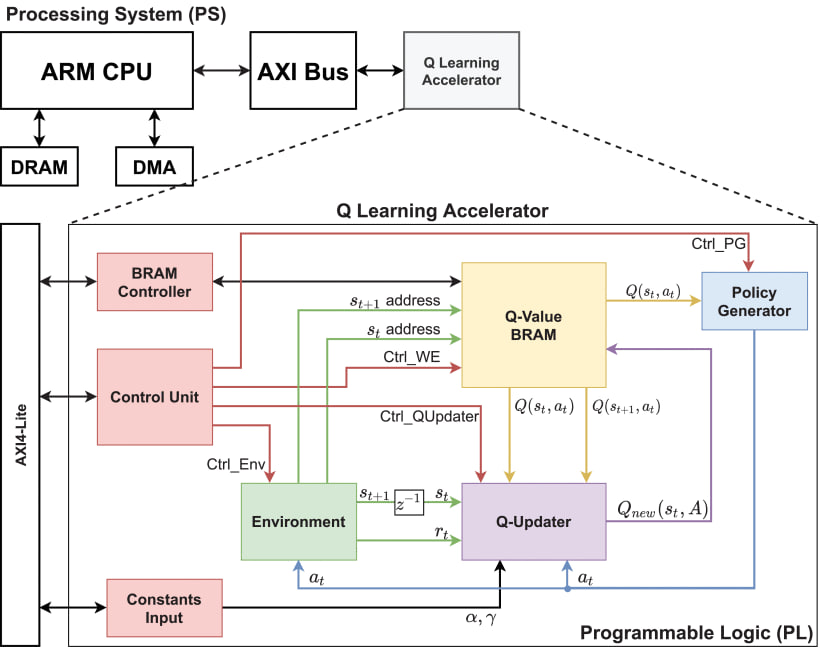
\includegraphics[width=0.8\textwidth]{chapter-2/faraneq.jpg}
	\caption{Ilustrasi arsitektur keseluruhan dari \parencite{sutisna2023faraneq}}
	\label{fig:ilustrasi-faraneq}
\end{figure}

Desain dari akselerator yang diajukan oleh \parencite{sutisna2023faraneq, dasilva2019parallel, panda2012FPGA} merupakan desain yang menggunakan prinsip separasi perangkat keras dan perangkat lunak menggunakan sistem \textit{Processing Systems-Processing Logic} (PS-PL) yang menghubungkan sebuah \textit{processor} sebagai PL dengan akselerator sebagai PS menggunakan sebuah bus dengan protokol tertentu, misalnya \textit{Advanced eXtensible Interface} (AXI) yang digunakan oleh \parencite{sutisna2023faraneq}.

Salah satu alternatif dari pendekatan desain PS-PL untuk mendesain akselerator adalah menggunakan ekstensi \ac{ISA}. \ac{ISA} adalah sebuah set instruksi yang ditentukan oleh sebuah arsitektur komputer yang menentukan perintah-perintah dasar yang dapat dilakukan oleh sebuah \textit{processor}. Riset yang dilakukan oleh Yang et al \parencite{yang2023design} adalah satu contoh penggunaan RISC-V untuk pengembangan akselerator perangkat keras. Akselerator pada \parencite{yang2023design} didesain untuk proses enkripsi pada perangkat \ac{IoT} dengan konsumsi daya rendah. Gambar \ref{fig:ilustrasi-lowiot} merupakan ilustrasi dari desain akselerator ekstensi \textit{processor} RISC-V pada \parencite{yang2023design}.

\begin{figure}[H]
	\centering
	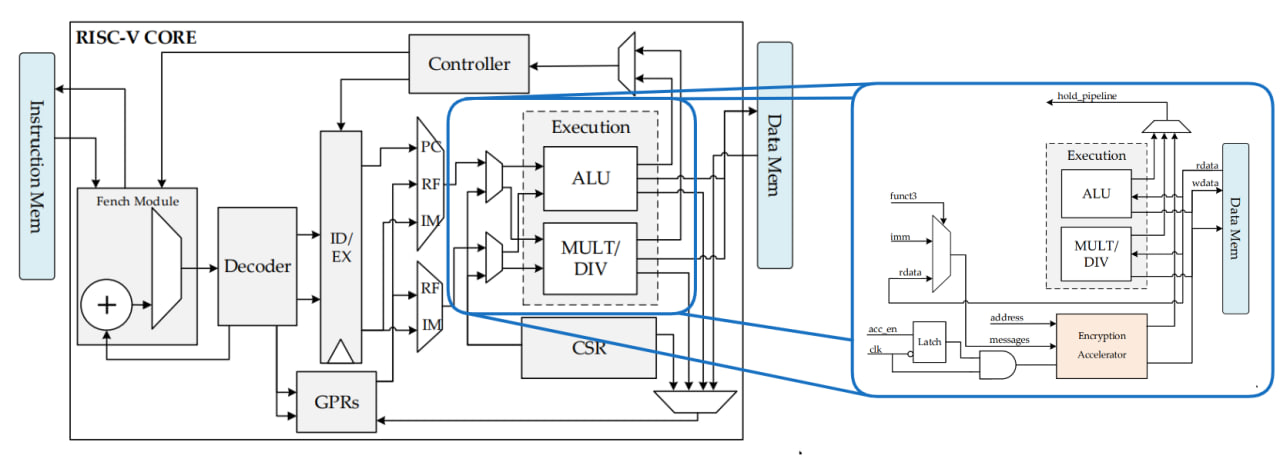
\includegraphics[width=1\textwidth]{chapter-2/lowiot.jpg}
	\caption{Arsitektur \textit{processor} RISC-V pada \parencite{yang2023design}}
	\label{fig:ilustrasi-lowiot}
\end{figure}

Kelebihan utama yang dimiliki oleh desain \parencite{yang2023design} adalah minimnya total penggunaan sumber daya perangkat keras dan minimnya \textit{delay} yang muncul dari transmisi data dari PS ke PL. Perancangan desain akselerator \ac{RL} yang menggunakan pendekatan sama dengan \parencite{yang2023design}, sampai penulisan tugas akhir ini, masih belum dilakukan. Sehingga, menjadi salah satu movitasi utama untuk melakukan eksplorasi desain akselerator \ac{RL} menggunakan \textit{processor} RISC-V.
